\documentclass{report}
\usepackage[utf8]{inputenc}
\usepackage[ngerman]{babel}
\usepackage{graphicx}
\usepackage{float}
\usepackage{commath}
\usepackage{hyperref}


\let\emph\relax % there's no \RedeclareTextFontCommand
\DeclareTextFontCommand{\emph}{\bfseries}

\newcommand{\UU}{\ensuremath{\underline{U}}}
\newcommand{\ugamma}{\ensuremath{\underline{\gamma}}}
\newcommand{\UUh}{\ensuremath{\UU_{h0}}}

\newcommand{\II}{\ensuremath{\underline{I}}}

\newcommand{\ZZ}{\ensuremath{\underline{Z}}}


\title{Einführung in die Hochfrequenz-Übertragungstechnik}
\author{Jonas Otto}
\date{März 2020}

\begin{document}

\tableofcontents
\maketitle

\chapter{Wellen}

\chapter{Leitungen}
\begin{figure}[H]
    \centering
    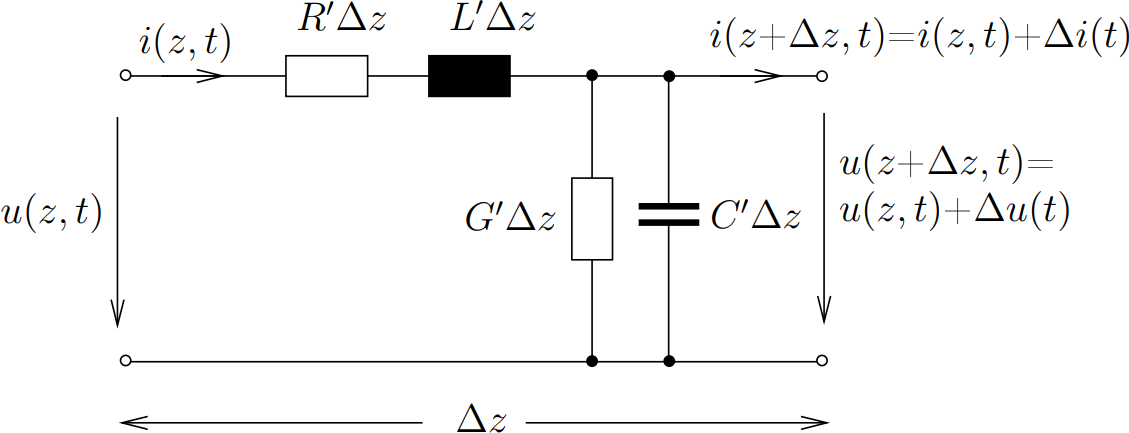
\includegraphics[width=\textwidth]{images/leitung.png}
    \caption{Infinitesimal kurzes TEM-Leitungsstück.}
\end{figure}

\section{Parameter Leitung}
Infinitesimales Leitungsstück kann mit Ersatzschaltbild mit Bauteilgrößen dargestellt werden:
\begin{description}
    \item[$R'$] \emph{Widerstandbelag}
    \item[$L'$] \emph{Induktivitätsbelag}
    \item[$G'$] \emph{Leitwertsbelag}
    \item[$C'$] \emph{Kapazitätsbelag}
\end{description}
Jeweils pro Längeneinheit.

Mittels komplexer Wechselstromrechnung und Kirchhoffschen Gesetzen ergibt sich die \emph{Telegrafengleichung}:
\begin{equation}
    \tag{Telegrafengleichung}
    \od[2]{\UU}{z} = \underline{\gamma^2}\UU
    \label{eqn:Telegraf}
\end{equation}
mit
\begin{equation}
    \tag{Gamma}
    \ugamma := \sqrt{\left(R'+j\omega L'\right)\left(G'+j\omega C'\right)} = \alpha + j\beta = j\underline{k}_z
    \label{eqn:gamma}
\end{equation}

Die Spannung lässt sich als Überlagerung einer hin- und zurücklaufenden Welle interpretieren:
\begin{equation}
    \boxed{ \UU(z)=\UU_h(z)+\UU_r(z) = \UUh e^{-\ugamma z}+\UU_{r0} e^{\ugamma}z }
\label{eqn:u-uberlagerung}
\end{equation}
\begin{equation}
    \boxed{ \II(z)=\frac{1}{Z_0} \left( \UU_h(z)-\UU_r(z)\right) = \frac{1}{Z_0} \left( \UUh e^{-\ugamma z}-\UU_{r0} e^{\ugamma}z \right) }
\label{eqn:i-uberlagerung}
\end{equation}

$\implies$ Der \emph{Ausbreitungskoeffizient $\gamma$} enthält alle Leitungsparameter.
Bei verlustloser Leitung besteht dies nur aus dem \emph{Phasenkoeffizient $\beta$}, da dann der \emph{Dämpfungskoeffizient $\alpha$} $= 0$ ist.

Damit lässt sich der \emph{Wellenwiderstand $Z_0$} berechnen:
\begin{equation}
    \underline{Z}_0 := \frac{R'+j\omega L'}{\ugamma} = \sqrt{\frac{R'+j\omega L'}{G'+j\omega C'}}
\end{equation}



\section{Leitung mit Abschlussimpedanz}
\begin{figure}[H]
    \centering
    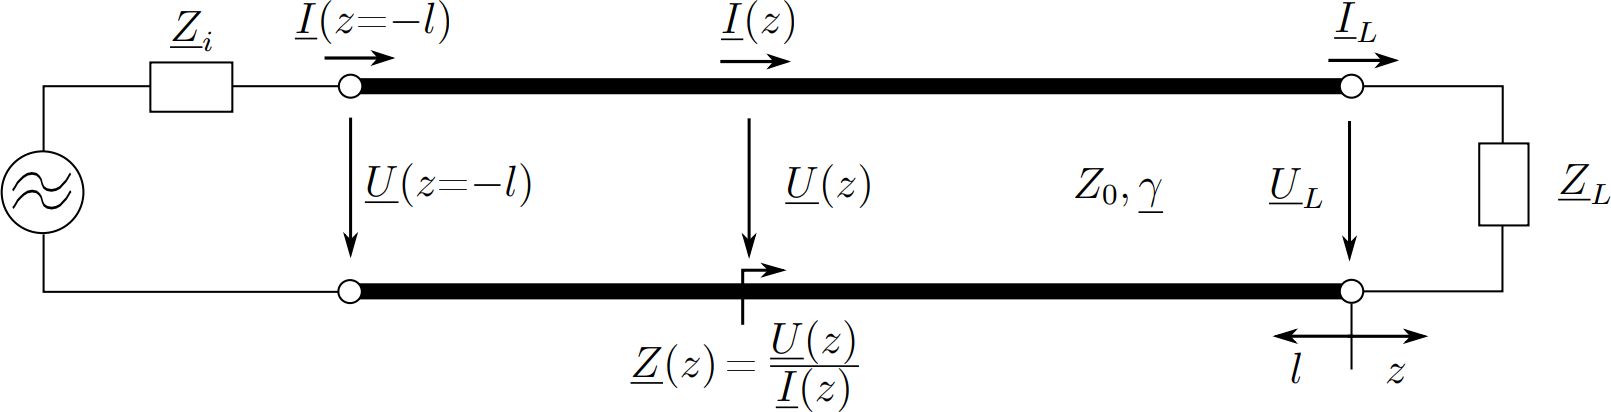
\includegraphics[width=\textwidth]{images/leitung_abschlussimpedanz.png}
\end{figure}
Hier sind Strom und Spannung am Ende der Leitung ($z=0$) bekannt: $\UU(z=0)=\UU_L$ und $\underline{I}(z=0)=\underline{I}_L$.

Mit diesen Randbedingungen lassen sich $\UUh$ und $\UU_{r0}$ bestimmen:
\begin{equation*}
    \UU(z=0) = \UUh + \UU_{r0} = \UU_L
\end{equation*}
\begin{equation*}
    \underline{I}(z=0) = \frac{1}{Z_0} (\UUh - \UU_{r0}) = \underline{I}_L
\end{equation*}

\begin{align}
    \implies \UUh &= \frac{1}{2} (\UU_L + Z_0 \underline{I}_L)\\
    \implies \UU_{r0} &= \frac{1}{2} (\UU_L - Z_0 \underline{I}_L)
\end{align}

Einsetzen in \eqref{eqn:u-uberlagerung} ergibt
\begin{equation}
    \UU(z) = \underbrace{ \frac{1}{2} \UU_L \left( 1 + \frac{Z_0}{\underline{Z}_L} \right) e^{-\ugamma z} }_{\text{Hinlaufend}} + \underbrace{ \frac{1}{2} \UU_L \left( 1 - \frac{Z_0}{\underline{Z}_L} \right) e^{\ugamma z} }_{\text{Rücklaufend}}
    \label{eqn:u-uberlagerung-z}
\end{equation}
\begin{equation}
    \II(z) = \underbrace{ \frac{1}{2} \frac{\UU_L}{Z_0} \left( 1 + \frac{Z_0}{\underline{Z}_L} \right) e^{-\ugamma z} }_{\text{Hinlaufend}} - \underbrace{ \frac{1}{2} \frac{\UU_L}{Z_0} \left( 1 - \frac{Z_0}{\underline{Z}_L} \right) e^{\ugamma z} }_{\text{Rücklaufend}}
    \label{eqn:i-uberlagerung-z}
\end{equation}

\noindent
Durch Division und Identitäten für $\cosh, \sinh$ ergibt sich:
\begin{equation}
    \ZZ(z) = \frac{\UU(z)}{\II(z)} = Z_0 \frac{\ZZ_L-Z_0 \tanh(\ugamma z)}{Z_0 - \ZZ_L \tanh(\ugamma z)}
\end{equation}

\subsection{Reflexionsfaktor}
Der \emph{Reflexionsfaktor $r$ an Stelle $z$} ist definiert als
\begin{equation}
    \tag{Reflexionsfaktor}
    \underline{r}(z) := \frac{\UU_r(z)}{\UU_h(z)} = - \frac{\underline{I}_r(z)}{\underline{I}_h(z)}
\end{equation}
Mit \eqref{eqn:u-uberlagerung-z} und $z=-l$ ergibt sich
\begin{equation}
    \underline{r}(l) = \frac{\underline{Z}_L-Z_0}{\underline{Z}_L+Z_0} e^{2\ugamma z} = \underline{r}(0) e^{-2\ugamma l}
\end{equation}
Beziehungsweise:
\begin{equation}
   \underline{r}(l) = \frac{\underline{Z}(l)-Z_0}{\underline{Z}(l)+Z_0} 
\end{equation}
\noindent
Für verlustlose Leitungen wird zusätzlich der \emph{SWR} definiert:
\begin{equation}
    \tag{VSWR}
    s := \left| \frac{\UU_\text{max}}{\UU_\text{min}} \right| = \frac{1+|\underline{r}|}{1-|\underline{r}|}
\end{equation}
Das Inverse davon nennt man \emph{Anpassungsfaktor}:
\begin{equation}
    \tag{Anpassungsfaktor}
    m := \frac{1}{s}
\end{equation}
Nützlich ist die Spannung als Funktion des Reflexionsfaktors bei $z=0$.
\begin{equation}
    \begin{aligned}
        \UU(z) &= \UU_h(z)(1+\underline{r}(z))\\
                         &= \UU_h(z)\left(1+\underline{r}(0) e^{2\ugamma z}\right)
    \end{aligned}
    \label{eqn:u-r}
\end{equation}
Für den Strom:
\begin{equation}
    \begin{aligned}
        \II(z) &= \frac{\UU_h(z)}{Z_0}(1-\underline{r}(z))\\
                         &= \frac{\UU_h(z)}{Z_0}\left(1-\underline{r}(0) e^{2\ugamma z}\right)
    \end{aligned}
    \label{eqn:i-r}
\end{equation}

Da bei der verlustlosen Leitung $\ugamma$ rein imaginär ist \eqref{eqn:gamma}, ist der Betrag von $\underline{r}$ dort unabhängig von $z$.

\subsection{Sonderfälle}
\begin{enumerate}
    \item \emph{Anpassung} ($Z_L = Z_0$)\\
        $\underline{r} = 0$, daraus folgt $\underbar{U}=\UU_h(z)=\UUh e^{-\ugamma z}$\\
        $s=1$\\
        In diesem Fall gibt es keine rücklaufende Welle, die Einhüllende entspricht also einer waagerechten Geraden mit Amplitude $|\UUh|$.
    \item \emph{Leerlauf} ($\underline{Z}_L \to \infty$)\\
        $r(0) = 1$, $s \to \infty$\\
        Mit $U_h(z) = \UUh e^{-\ugamma z}$ \eqref{eqn:u-uberlagerung}
        und $\UU(z)=\UU_h(z)\left(1+\underline{r}(0) e^{2\ugamma z}\right)$
        \eqref{eqn:u-r} ergibt sich
        $\UU(z) = \UUh\left( e^{-\ugamma z} + e^{\ugamma z} \right) =2 \UUh \cosh(\ugamma z)$\\
        mit $\alpha=0 \implies \UU(z)=2 \UUh \cos(\beta )$\\
        $\implies$ Stehende Welle\\
        Strom: mit \eqref{eqn:i-r} und $\UU_h$ (siehe oben):\\
        $\implies \II(z)=-2j\frac{\UUh}{Z_0}\sin(\beta z)$\\
        $\ZZ(z) = \frac{\UU(z)}{\II(z)} = -Z_0\coth(\ugamma z)$\\
        Für $l \ll \lambda$ wirkt eine offene Leitung wie eine Kapazität.
        
    \item \emph{Kurzschluss} ($Z_L=0$)\\
        $r(0) = -1, s=\infty$\\
        $\implies$ Wieder stehende Welle\\
        Bei $l \ll \lambda$ verhält sich die kurzgeschlossene Leitung wie eine Induktivität.
        
    \item \emph{$l = \frac{\lambda}{4}$} $\frac{\lambda}{4}$-Transformator ($\underline{Z}_L$ beliebig)\\
        $\underline{Z}(l=\frac{\lambda}{4})=\frac{Z_0^2}{Z_L}$\\
        Wandelt z.B. Kurzschluss und Leerlauf ineinander um.

    \item \emph{$l = \frac{\lambda}{2}$} ($\ZZ_L$ beliebig)\\
        $\ZZ(l=\frac{\lambda}{2}) = \ZZ_L$\\
        $\implies$ Einfügen einer Leitung mit Länge $\frac{\lambda}{2}$ hat keinen Einfluss wenn die Leitung verlustlos und die Frequenz konstant ist.
\end{enumerate}


\chapter{Smith-Diagramm}

\chapter{Streumatrix}

\chapter{Rauschen}

\chapter{Komponenten}

\chapter{Übertragungssysteme}

\chapter{Modulation}

\chapter{Wellenausbreitung}

\end{document}

